\documentclass[10pt]{article}

\usepackage{balance}
\usepackage[margin=1.0in]{geometry}
\usepackage{graphicx}
\usepackage{ifpdf,theorem,tabularx,multirow}

\newcommand{\ie}{{\em i.e.,}~}
\newcommand{\eg}{{\em e.g.,}~}

\begin{document}
\title{ICDM 2013 Outline}
%\author{Kristal Curtis}
\maketitle

\abstract

\section{Introduction (1)} 

\begin{itemize}
\item{Short read data is proliferating as sequencing costs fall faster than Moore's Law.}
\item{Analyzing the short read data remains the major challenge to making use of this data [citation saying that analysis cost dominates sequencing cost].}
\item{One way to reduce the computational demands of processing short read data is to use a simple, efficient approach whenever possible, focusing expensive and more accurate techniques only where necessary [cite Biggie workshop paper].}
\item{The main task we must accomplish before pursuing this approach is to identify which regions of the genome require the more advanced approach.}
\item{One of the main challenges to processing genomic data is the genome's structure itself, namely, the similar regions.}
\item{Existing approaches to identifying similar regions are ill-suited to our problem; they're more focused on understanding the biology/evolutionary history of the sequence.}
\item{We've developed a novel way of identifying the similar regions, and we demonstrate that the similar regions we've identified correlate with the regions where processing is difficult.}
\item{We demonstrate our results on both simulated and real data.}
\end{itemize}

\section{Background (1)}

\subsection{Short reads (0.25)}
\begin{itemize}
\item{Since we can't read off the entire genome in one long string, we split the DNA into fragments and then read off the sequence on each end.  (3B characters long; possible characters are A, C, G, T)}
\end{itemize}
\subsection{Alignment (0.25)}
% Will cite BWA, Bowtie2, SNAP, ...
\begin{itemize}
\item{We get lots of short reads from the sequencer, and we want to figure out how to reconstruct the full genome from the reads.}
\item{Instead of starting from scratch (like putting a puzzle together), we do alignment (like looking at the picture on the box cover).}
\end{itemize}
\subsection{Variant calling (0.25)}
% Will cite GATK, Samtools (mpileup)
\begin{itemize}
\item{Once we have aligned all the reads, we want to get back the original genome.}
\item{A genome can be expressed as a set of variants from the reference genome; since people are highly similar (99.9\%), the set of variants is not too large.}
\item{Variant calling is accomplished basically by considering all the reads at a given location and then determining the consensus about what the reads say the sample genome contains at that location.}
\end{itemize}
Cite Figure \ref{fig:variantCallingOverview}.
\begin{figure}
\centering
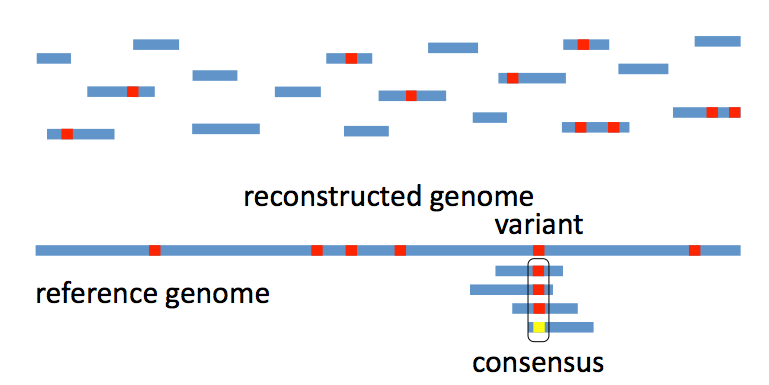
\includegraphics[scale=0.5]{variantCallingOverview}
\caption{Variant calling overview:  short reads are produced by the sequencer, which are then aligned to the reference genome.  Variant calling basically determines the consensus among the reads overlapping each position in the genome.  The reconstructed genome is the set of variants produced.}
\label{fig:variantCallingOverview}
\end{figure}

\section{The Problem of Similarity (1.5)}
\begin{itemize}
\item{If the genome were a random string of 3B bases long, the alignment problem would be easy (calculate odds of getting the right spot).}
\item{However, the genome is actually characterized by both exact and near duplication.}
\item{Exact \& near duplication in the genome is not just trivial patterns (no, it's not just a bunch of AAAAAAs).}\\
** Figure showing some example duplicate, near-duplicate strings
\item{Exact duplication is an easy problem to deal with:  (1) you can easily locate exact-duplicate regions, and (2) since there is no unambiguous answer as to where a read of this sort comes from, you can just mark it as ambiguous and move on.}
\item{Near duplication is a much more difficult problem, since:  (1) locating near-duplicate regions is much more difficult, and (2) since there \_is\_ often an unambiguous best answer to where reads from these regions originated, you need to spend a lot of time matching the reads against all the possible locations to find the best one.}\\
** Generate reads from \& align reads to repeat masked genome vs. full genome -- want to show that both runtime \& accuracy suffer when near-duplication is present
\item{Alignment errors caused by near duplication can lead to variant calling errors.}\\
Cite Figure \ref{fig:problemOfSimilarity}.
\end{itemize}
\begin{figure}
\centering
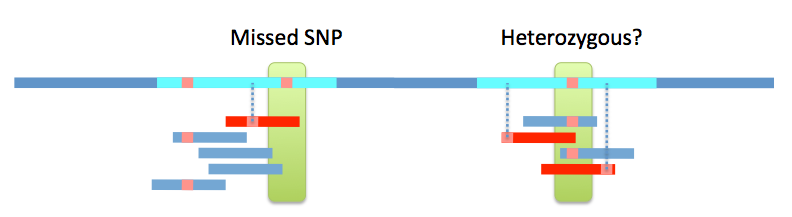
\includegraphics[scale=0.5]{problemOfSimilarity}
\caption{The problem of similarity.}
\label{fig:problemOfSimilarity}
\end{figure}

\section{Similar Region Detection (2)}

\begin{itemize}
\item{Our approach to finding the similar regions is driven by the short reads themselves (look at substrings of genome that are the same length as the reads).}
\item{We employ an offline approach using the union find algorithm.}
\begin{itemize}
\item{Basic recap of union find}
\item{Explain how to apply union find to our setting}\\
Cite Figure \ref{fig:unionFind}.
\begin{figure}
\centering
\begin{tabular}{c c}
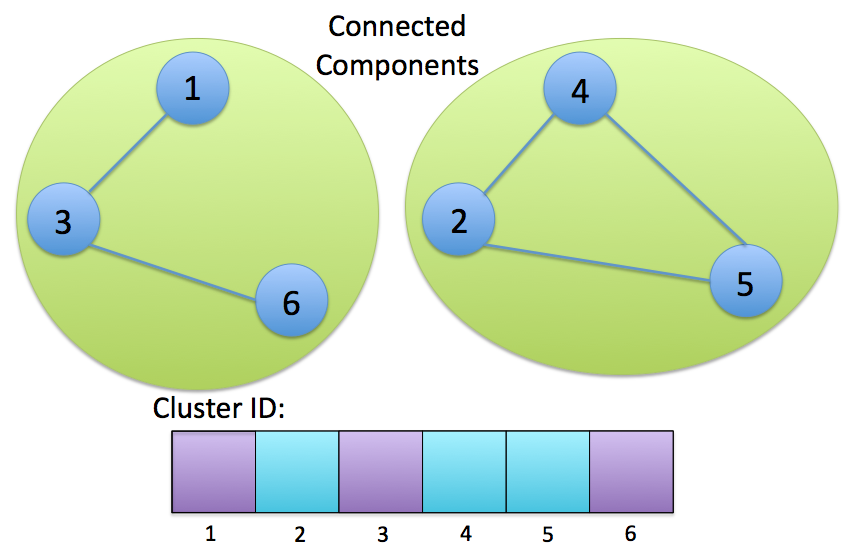
\includegraphics[scale=0.25]{basicUnionFind} & 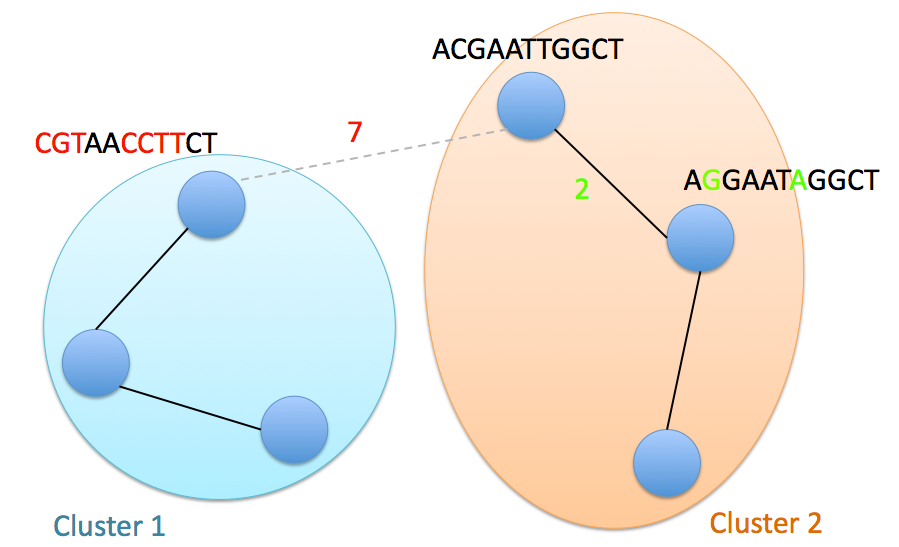
\includegraphics[scale=0.25]{applyingUnionFind}
\end{tabular}
\caption{(a) Basic union find.  (b)  Applying union find to genome substrings.}
\label{fig:unionFind}
\end{figure}
\end{itemize}
\item{Since there are 3B substrings of length 100 in the genome, we need several optimizations to make this computation tractable.}
\begin{itemize}
\item{Motivate why you care about runtime:  development, want to try different parameter settings, want to redo when you get new read lengths/read technologies.}
\item{Usually, you want the full adjacency matrix, where there is an edge between any sufficiently similar substrings.}
\item{Instead of doing the full 3Bx3B comparisons, we use an index to find similar substrings.}\\
Cite Figure \ref{fig:implementingUnionFind}.
\begin{figure}
\centering
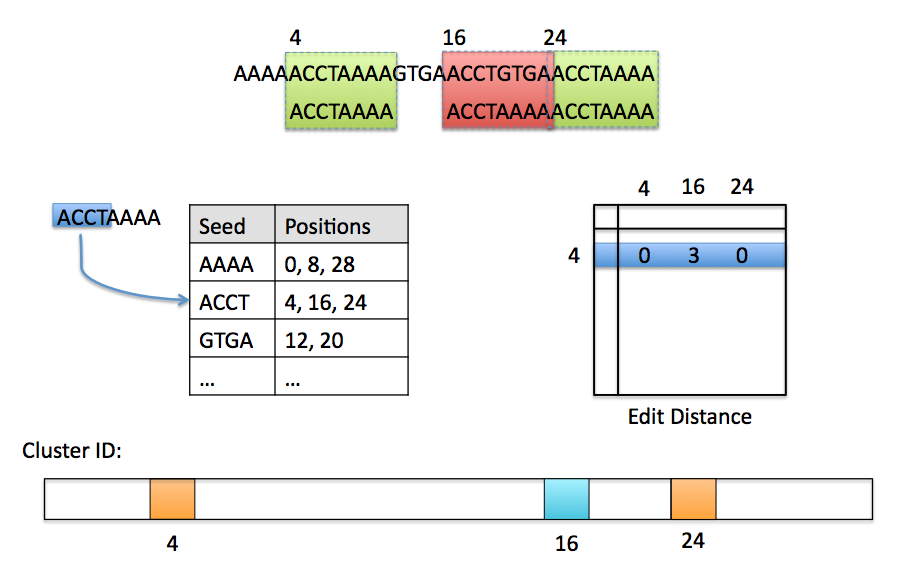
\includegraphics[scale=0.4]{implementingUnionFind}
\caption{Implementing union find.}
\label{fig:implementingUnionFind}
\end{figure}
\end{itemize}
\item{This is still a lot of comparisons, so we need a parallel implementation to make this finish in a reasonable amount of time.}
\begin{itemize}
\item{We use Spark.}
\item{We experimented with different partitioning schemes, and we ended up choosing a grid partitioning.}
\item{Grid partitioning complicates how you do the merging.}\\
Cite Figure \ref{fig:parallelUnionFind}.
\begin{figure}
\centering
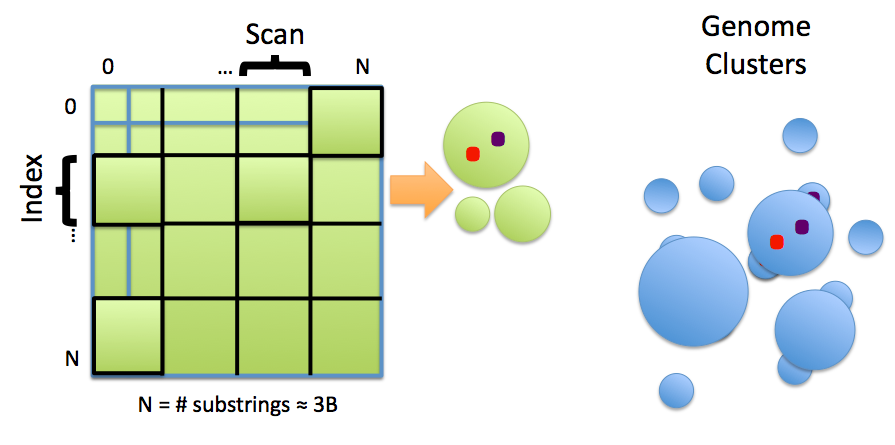
\includegraphics[scale=0.4]{parallelUnionFind}
\caption{Parallelization of union find.}
\label{fig:parallelUnionFind}
\end{figure}
\end{itemize}
\end{itemize}

\section{Experiments (3)}

\begin{itemize}
\item{Info about how similar region finder works (setup, runtime, resource requirements, etc.)}
\item{Similar regions correlate with alignment errors (easy/hard reads, with multiple aligners) for both synthetic \& real data (will have to look at aligner agreement instead of alignment errors)}\\
Cite Figure \ref{fig:errorsInClustersGraph}.\\
\begin{figure}
\centering
\begin{tabular}{c c}
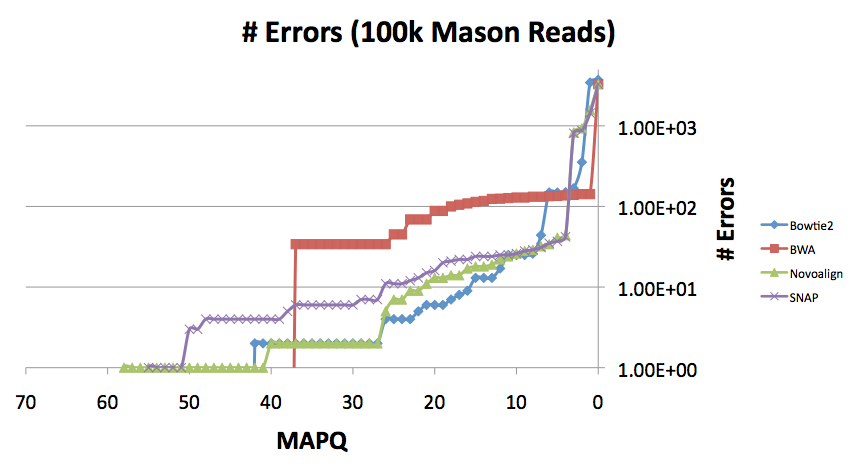
\includegraphics[scale=0.3]{errorsByMapq} & 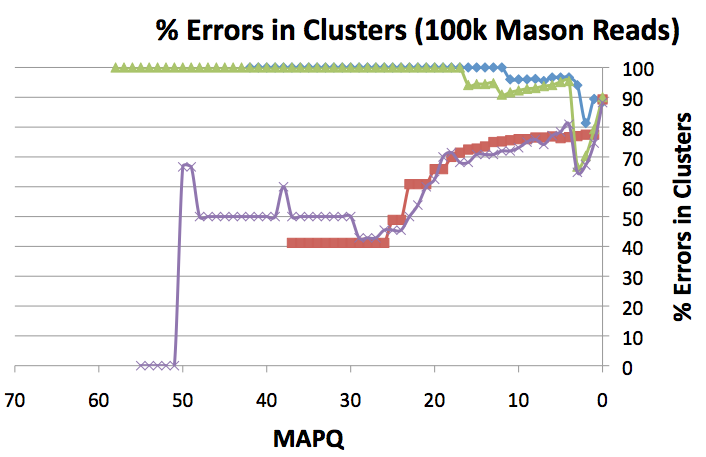
\includegraphics[scale=0.3]{errorsInClusters}
\end{tabular}
\caption{(a) Errors by MAPQ for each of 4 aligners.  (b) Errors in clusters by MAPQ.  At all MAPQ, a large fraction of errors are in clusters for all 4 aligners.}
\label{fig:errorsInClustersGraph}
\end{figure}
% this should eventually be a latex table
Cite Table \ref{table:alignerAgreement}.\\
\begin{figure}
\centering
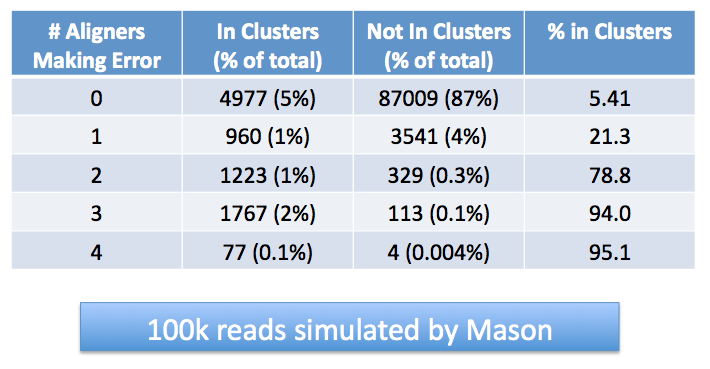
\includegraphics[scale=0.5]{alignerAgreementTable}
\caption{As reads get harder (\ie fewer aligners agree), reads are more likely to be in clusters.}
\label{table:alignerAgreement}
\end{figure}
** Show how often, for the simulated data, aligner agreement corresponds to all 4 aligners being correct -- ie, when all 4 aligners agree, how often are they correct?  Gives basis for using this metric with real data.\\
\item{End-to-end analysis:  Show that variant calling is easier with regions of the genome that are NOT in clusters (for both synthetic \& real data -- use SMASH)}
\begin{itemize}
\item{Reads \(=>\) aligned reads (with BWA) \(=>\) variant calls (with mpileup)}
\item{Compute VC accuracy on all calls}
\item{Compute VC accuracy after filtering out calls in similar regions -- show that this is better than accuracy on all calls \(=>\) demonstrates that VC is harder in similar regions}
\end{itemize}
** Table showing VC accuracy overall vs. just in unique regions
\end{itemize}

\section{Related Work (0.5)}

\begin{itemize}
\item{Finding repeats in the genome -- their goal (find all kinds of repeats) is different \& therefore so is their approach; their approach covers a large portion of the genome}
\item{Clustering DNA sequences (metagenomics) -- their goal (find all reads from one species) is different \& therefore the clusters these algorithms produce are not useful for us}
\item{MAQ paper on using MAPQ to indicate ``hard" reads -- want to show that my approach is better at identifying hard regions}
\item{Review paper on how aligners handle repeat regions}
\item{Biggie idea of separating into easy/hard regions}
\end{itemize}

\section{Conclusions \& Future Work (0.5)}

\begin{itemize}
\item{Efficiently and accurately reconstructing a sample genome from short read data is a very important and challenging problem (precondition to clinical usage of genomic data).}
\item{We suggest that to obtain an efficient solution without sacrificing accuracy, a hybrid approach should be employed in which simple variant calling techniques are applied to easy regions and more advanced techniques are applied only where necessary.}
\item{The structure of the genome is what makes this analysis difficult.}
\item{We have developed a novel definition of similar regions that is driven by the short reads themselves, and we have developed a scalable approach to detect them.}
\item{We have established that our similar regions correspond to the hard regions of the genome.}
\item{We have presented evidence that our hybrid approach will be an efficient \& accurate VC approach.}
\item{Future Work:}
\begin{itemize}
\item{Reduce false positives/hone in on similar regions that correspond to where aligners have difficulty (right now it's 10\% of the genome, but should probably be more like 5\%).}
\item{Develop system that applies simple techniques to unique regions \& advanced techniques to similar regions to obtain highly accurate VC efficiently.}
\end{itemize}
\end{itemize}

\section*{References (0.75)}

\end{document}